\documentclass[tikz, margin=3.14mm]{standalone}
\usepackage{pgfplots}
\usetikzlibrary{arrows.meta, backgrounds}
\pgfplotsset{compat=1.18}

\begin{document}
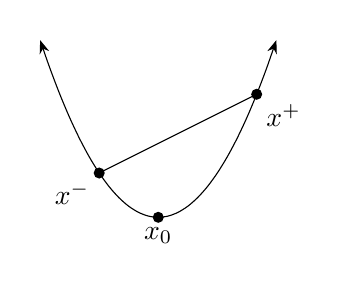
\begin{tikzpicture}[
    background rectangle/.style={fill=white}, 
    show background rectangle]
    % Define the two points A and B
    \coordinate (A) at (-.75, .5625);
    \coordinate (B) at (1.25, 1.5625);
  
    % Draw the parabola y = x^2
    \draw[Stealth-Stealth, domain=-1.5:1.5, smooth] plot (\x, \x*\x);
  
    % Highlight the points A and B
    \fill (A) circle (2pt);
    \fill (B) circle (2pt);
    \fill (0,0) circle (2pt);
  
    % Draw a line connecting A and B
    \draw (A) -- (B);
  
    % Optionally, you can label the points
    \node[below left] at (A) {$x^-$};
    \node[below right] at (B) {$x^+$};
    \node[below] at (0,0) {$x_0$};
  \end{tikzpicture}
\end{document}